% !TeX spellcheck = fr_FR
\documentclass[french]{yLectureNote}

\title{Introduction à la thermodynamique}
\subtitle{Thermodynamique}
\author{Paulhenry Saux}
\date{\today}
\yLanguage{Français}

\professor{}

\usepackage{graphicx}%----pour mettre des images
\usepackage[utf8]{inputenc}%---encodage
\usepackage{geometry}%---pour modifier les tailles et mettre a4paper
%\usepackage{awesomebox}%---pour les boites d'exercices, de pbq et de croquis ---d\'esactiv\'e pour les TP de PC
\usepackage{tikz}%---pour deiffner + d\'ependance de chemfig
\usepackage{tkz-tab}
\usepackage{tabularx}%---pour dimensionner automatiquement les tableaux avec variable X
\usepackage{awesomebox}%---Pour les boites info, danger et autres
\usepackage{menukeys}%---Pour deiffner les touches de Calculatrice
\usepackage{fancyhdr}%---pour les en-t\^ete personnalis\'ees
\usepackage{blindtext}%---pour les liens
\usepackage{hyperref}%---pour les liens (\`a mettre en dernier)
\usepackage{caption}%---pour la francisation de la l\'egende table vers Tableau
\usepackage{pifont}
\usepackage{array}%---pour les tableaux
\usepackage{lipsum}
\usepackage{yFlatTable}
\usepackage{multicol}
\newcommand{\Lim}[1]{\lim\limits_{\substack{#1}}\:}
\renewcommand{\vec}{\overrightarrow}
\newcommand{\bz}{\overline{z}}
\DeclareMathOperator{\card}{card}
\renewcommand{\vec}{\overrightarrow}
\newcommand{\N}[0]{\mathbb{N}}
\newcommand{\R}[0]{\mathbb{R}}
\newcommand{\C}[0]{\mathbb{C}}
\newcommand{\dd}[0]{\mathrm{d}}
\newcommand{\er}{\vec{e_{\rho}}}
\newcommand{\ep}{\vec{e_{\varphi}}}
\newcommand{\pip}{\pi^+}
\newcommand{\pim}{\pi^-}
\newcommand{\mv}{\mathcal{V}}
\DeclareMathOperator{\Div}{Div}
\newcommand{\rot}{\vec{\mathrm{rot}}}
\newcommand{\grad}{\vec{\mathrm{grad}}}
\begin{document}
\chapter{Définitions}
\subsection{Introduction}
Dans tout ce que l'on va étudier, le système sera dans un état d'équilibre au départ et à la fin\marginCheck{Ce n'est pas le cas d'une tasse chaude posée à l'extérieur, car ce n'est pas à l'équilibre}.

On ne mélangera pas les corpus ou échelles. Ici, ce n'est pas en microscopique
\section{Les états de la matière}
\begin{itemize}
    \item solide (parfois incompressible indéformant par hypothèses)
    \item liquide (prend la forme du réservoir qui le contient)
    \item gazeux (occupe tout le volume disponible)
\end{itemize}
On les différencie par leur propriété
\section{Système thermodynamique}
La première chose à faire est de s'interroger sur le système (type, frontières) que l'on est en train d'étudier.
\begin{definition}[Système thermodynamique]
    Ensemble matériel impliqué dans une processus de conversion d'énergie. 
    Il peut \^etre délimité par des frontière fixes ou mobiles réelles ou imaginaires
\end{definition}
\checkInfo{Exemple : Bouteille Thermos}{On étudie le café, un liquide, ou les paroies, un solide}
On définit 3 sortes de systèmes :
\begin{itemize}
    \item Système isolé : C'est le cas d'un système indéformable avec un isolant parfait autour
    \item  Système fermé : C'est le cas d'une pompe à vélo avec le trou bouché
    \item Système ouvert
\end{itemize}
\begin{definition}[Système isolé]
    N'échnage ni matière ni énergie avec l'extérieur du système. Cela peut dépendre du temps d'observation. 
    L'intérieur est appelé univers thermodynamique. L'extérieur est le reste de notre univers.
\end{definition}

\begin{definition}[Système fermé]
    Il n'y a pas de transfert de matière mais échange d'énergie. La masse est constante
\end{definition}
\begin{definition}[Système ouvert]
    Échange matière et énergie avec le reste de l'univers
\end{definition}
\section{Variables}
\begin{definition}[Variable thermodynamique]
    Toute grandeur variant, mesurable, directement ou non, appartenant au système
\end{definition}
On distingue 2 types de variables :
\begin{itemize}
    \item variables extensives : m, v, n, E
    \item variables intensives : P, T
\end{itemize}
\begin{definition}[Densité massique d'une grandeur extensive]
    Soit Y une grandeur extensive. On définit $$y = \Lim{m\to 0}\frac{Y}{m}$$ qui est une grandeur intensive.
\end{definition}
C'est utile quand on veut définir une grandeur définie localement.
\begin{theorem}
    Pour un système fermé contenant un corps pur, l'état est connu si 2 variables thermodynamiques, souvent (P,T), (P,V), (T,V).
\end{theorem}
\section{Notion de température}
\begin{definition}[Température]
    La grandeur que partagent 2 systèmes en équilibre thermique
\end{definition}
\begin{theorem}[Passage d'une unité à l'autre]
    \begin{itemize}
        \item $T[F] = \frac95 T[C]+32$
        \item $T[K] = T[C]+273.15$
    \end{itemize}
\end{theorem}
\begin{definition}[Température cinétique (corpus microscopique)]
    Vitesse quadratique moyenne de la translation des molécules
\end{definition}
\section{Pression}
\begin{definition}[Pression]
    Notée $p$, elle s'exprime en Pascal et correspond à la densité de force qu'exerce le gaz/liquide sur son contenant :$$\dd \vec{F} = p\vec{\dd S}$$
\end{definition}
\checkInfo{Autres unités}{$$ 1 atm = 101325 Pa, 1 bar = 10^5 Pa$$}
\subsection{Quelques lois de la statique des fluides}
\subsubsection{loi de l'hydrostatique}
Soit un élément de volume infinitésimal $dV = dx\,dy\,dz$ d'un fluide au repos :
\begin{itemize}
    \item $P(x,y,z)$ : Pression locale [Pa].
    \item $\rho$ : Masse volumique du fluide [kg.m$^{-3}$].
    \item $\vec{g}$ : Champ de pesanteur [m.s$^{-2}$].
\end{itemize}
À l'équilibre, le Principe Fondamental de la Dynamique ($\sum \vec{F} = \vec{0}$) donne :

\paragraph{Suivant l'axe horizontal ($x$) :}
\begin{equation}
P(x)dy\,dz - P(x+dx)dy\,dz = 0 \implies -\frac{\partial P}{\partial x} dx\,dy\,dz = 0 \implies \frac{\partial P}{\partial x} = 0
\end{equation}

\paragraph{Suivant l'axe vertical ($z$, ascendant) :}
En incluant le poids\marginWarning{Si $\vec{g} = \vec{0}$, l'équation d'équilibre implique $\vec{\text{grad}}(P) = \vec{0}$. 
Cela signifie que la pression est unforme (identique en tout point). La pesanteur n'invente pas la pression, elle crée un \textbf{gradient} : elle force le fluide à se "tasser", augmentant la pression avec la profondeur.} $d\vec{W} = \rho\,dV\vec{g}$ :
\begin{equation}
P(z)dx\,dy - P(z+dz)dx\,dy - \rho g \, dx\,dy\,dz = 0
\end{equation}
Par développement limité $P(z+dz) \approx P(z) + \frac{\partial P}{\partial z}dz$, puis en simplifiant par $dV$ :
\begin{equation}
-\frac{\partial P}{\partial z} - \rho g = 0 \implies \frac{\partial P}{\partial z} = -\rho g
\end{equation}

La généralisation aux trois dimensions donne la loi de l'hydrostatique :

\begin{theorem}[Loi de l'hydrostatique]
    $$\vec{\text{grad}}(P) = \rho \vec{g}$$
\end{theorem}

\subsubsection{Application aux gaz parfaits}
D'après la loi des gaz parfaits :
\begin{equation}
PV = nRT \implies P = \frac{m}{M \cdot V} RT \implies P = \rho \frac{RT}{M}
\end{equation}
Où $M$ est la masse molaire du gaz et $R$ la constante universelle des gaz parfaits. On en déduit :
\begin{equation}
\rho = \frac{P \cdot M}{RT}
\end{equation}

En substituant $\rho$ dans l'équation de la statique ($\frac{dP}{dz} = -\rho g$) :
$$
\frac{dP}{dz} = -\frac{PMg}{RT} \implies \frac{dP}{P} = -\frac{Mg}{RT} dz
$$
En intégrant entre deux altitudes $z_A$ et $z_B$ pour une température $T$ constante :
\begin{equation}
\int_{P(z_A)}^{P(z_B)} \frac{dP}{P} = \int_{z_A}^{z_B} -\frac{Mg}{RT} dz
\end{equation}
On obtient la loi du nivellement barométrique :
\begin{theorem}[Loi du nivellement barométrique]
    $$\ln\left(\frac{P(z_B)}{P(z_A)}\right) = -\frac{Mg}{RT}(z_B - z_A)$$
\end{theorem}

\section{Équilibre Thermodynamique}
\begin{definition}[Système à l'équilibre]
    Un système est à l'équilibre s'il n'y a pas de flux de masse, pas de flux d'énergie et que l'état est stationnaire.
\end{definition}

\section{Équation d'état}
Une équation d'état est une relation reliant les variables d'état à l'équilibre :
\begin{equation}
f(P, V, T) = 0
\end{equation}
\begin{definition}[Gaz parfait]
    Un gaz est dit parfait s'il respecte $PV = nRT$.
\end{definition}
Pour prendre en compte le volume propre des molécules ($b$) et leurs interactions ($a$)\marginCritical{En effet, le mdèle des gaz parfaits suppose que les interactions à distance entre molécules sont négligeables.}, on utilise :
\begin{definition}[Modèle de Van der Waals]
    Pour prendre en compte le volume propre des molécules ($b$) et leurs interactions ($a$), on utilise :
    $$\left( P + \frac{n^2 a}{V^2} \right) (V - nb) = nRT$$
\end{definition}

\section{Réservoir}

\begin{definition}[Thermostat/Réservoir/Source]
    C'est un lieu à qui on peut prendre ou donner de l'énergie autant que l'on veut sans que sa température ne change.
\end{definition}

\section{Transformations}
\begin{definition}[Transformation]
    Passage d'un système d'un état initial (d'équilibre) à un autre d'équilibre aussi.
\end{definition}
Exemple :
\begin{itemize}
    \item $\searrow$ \textbf{Volume} : compression
    \item $\nearrow$ \textbf{Volume} : détente
\end{itemize}

% Note : Le schéma sur le manuscrit représente un cylindre avec un piston mobile 
% contenant un gaz, souvent utilisé pour illustrer ces transformations.

\includegraphics[scale=0.5]{c1.pdf}

On écrit : $I\to F$ pour noter une transformation de l'état initial à l'état final.
\subsection{Transformations quasi-statique VS non quasi-statique}
\begin{definition}[Transformation Quasi-statique]
    C'est une transformation constituée par une succession continue d'états d'équilibre, quelque soit l'amplitude des variations que l'on fait. 
\end{definition}
C'est une succession continue d'état quasi-statique.\marginCritical{Pour atteindre l'équilibre, il faut un temps infiniment long. Les transformations quasi-statique n'existent pas dans la nature. }
\checkInfo{Exemple}{Par exemple, on ajoute un grain de sable, puis on attend une infinité de temps, puis on recommence}

\begin{definition}[Transformation non quasi-statique]
    Transorfamtion au coirs de la quelle au moins un état n'est pas des états d'équilibre.
\end{definition}
Nous étudions la variation de l'énergie du système, qui est une grandeur d'état. 
Peu importe les transformations intermédiaires. On peut donc inventer un chemin avec des états intermédiaires. 
On va donc imaginer des transformations quasi-statiques\marginInfo{De plus, Certaines transformations effectuées lentement pourront \^etre approchées par une transformation quasi-statique pour modéliser.}.

\begin{definition}[Transformation réversible]
    On peut faire la transformation dans le sens inverse, on obtient alors l'état initial, et la transformation a un sens physique.
\end{definition}
\subsection{Exemples}
% \subsubsection{Expérience 1}
% Un piston dans un cylindre avec des paroies non isolantes thermiquement\marginCritical{Perméables à la chaleur}, au niveau de la mer. Il y a une mole d'un gaz parfait dans le cylindre, dans un volume de 1L.
% Il y a une température extérieure de 20°. Le rayon a un rayon de 10cm. Le piston a un tas de sable de 7 tonnes au dessus de lui.

% État initial du Gaz\marginCritical{Par définition, le piston et le système ne bouge} (= Pression, Température, Volume) : $T_i = T_{atm} = 20°, V_i = 1L$

% Calculons la pression qu'exerce le gaz sur le piston : $P_i = \frac{nRT_i}{V_i} = 24.36\cdot 10^5 Pa.$.

% Si le gaz est à l'équilibre, son volume aussi, donc le piston ne bouge pas.

% On écrit\marginInfo{On ne peut pas négliger la masse du piston} le PFD : donc $P_iS_p-P_{atm}S_p -m_p g = 0$. On en déduit que $P_i = P_{atm}+\frac{m_p g}{S_p}$.

% On en déduit que la masse totale piston+sable est à 7480 Kg.

% On suppose que le piston est sans masse.

% Expérience (quasi-statique) : On enlève les grans de sable un par un.

% État final (quasi-statique) : Les parois sont perméables à la chaleur, on est à l'équilibre donc $P_f = P_{atm}$. De plus, $P_f = P_{atm}$ et $V_f = \frac{nRT_f}{P_f} = 24.36L$.

% La transformation est une détente isotherme.
% \warningInfo{Transformation isotherme}{C'est une transformation au cours de laquelle la température reste inchangée. De plus, Une isotherme sera toujours quasi-statique.}

% On représente avec un diagramme de Clapeyron
% %TODO Diagramme de Clapeyron fig 2

% Expérience (non quasi-statique). La température n'est pas définie de la m\^eme façon dans tout le gaz car les paroies ne sont pas adiabatiques.




\subsubsection{Expérience 1 : Détente isotherme quasi-statique}

\paragraph{Configuration initiale}
Un cylindre avec parois thermiquement perméables contient une mole de gaz parfait :
\begin{itemize}
    \item Volume initial : $V_i = 1\text{ L}$
    \item Température : $T_i = 20°\text{C}$ (température ambiante)
    \item Piston sans masse, rayon $r = 10\text{ cm}$
    \item Sable sur le piston : masse totale $m = 7\text{ t}$
\end{itemize}

\paragraph{État initial}
À l'équilibre, en appliquant le PFD sur le piston :
$$P_i S_p = P_{\mathrm{atm}} S_p + mg \implies P_i = P_{\mathrm{atm}} + \frac{mg}{S_p} \approx 24.36 \times 10^5 \text{ Pa}$$

Processus : enlever les grains de sable un par un\marginInfo{Cette succession d'états d'équilibre constitue une \textbf{transformation quasi-statique}.}

\paragraph{État final}
Les parois permettent l'équilibre thermique avec l'extérieur :
$$P_f = P_{\mathrm{atm}}, \quad T_f = 20°\text{C}$$
$$V_f = \frac{nRT_f}{P_f} = 24.36\text{ L}$$


La transformation $I \to F$ est une détente isotherme quasi-statique\marginTips{On aurait pu obtenir un processus non quasi-statique avec une autre expérience : On enlève le sable d'un coup. La température n'est pas définie de la m\^eme façon dans tout le gaz car les paroies ne sont pas adiabatiques.}.

À chaque instant : $T = \text{cte} = 20°\text{C}$


\warningInfo{Transformation isotherme}{C'est une transformation au cours de laquelle la température reste inchangée. De plus, Une isotherme sera toujours quasi-statique.}
\begin{definition}[Transformation monotherme]
    C'est une = transformation telle que $T_{ext} = T_i = T_f$
\end{definition}


On représente ces états avec un diagramme de Clapeyron

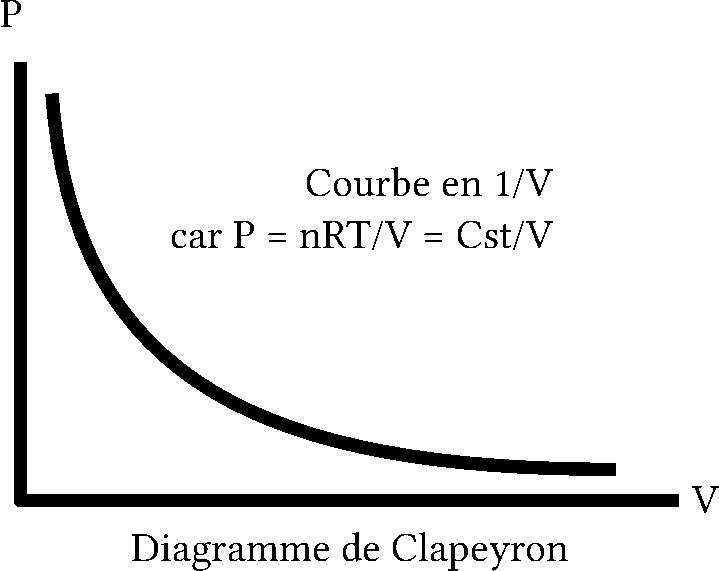
\includegraphics[scale=0.6]{clap.pdf}

\subsubsection{Expérience 2 : Refroidissement isobare non quasi-statique}

\paragraph{Configuration initiale}
Un cylindre avec piston dans une pièce à température ambiante :
\begin{itemize}
    \item Température initiale : $T_i = 20°\text{C}$
    \item Pression : $P_i = P_{\mathrm{atm}}$
    \item Volume initial : $V_i = \frac{nRT_i}{P_i} = 24.36\text{ L}$
\end{itemize}

\paragraph{Expérience : déplacement dans une pièce plus froide}
On déplace le système dans une pièce à température $T_{\mathrm{ext}} = 10°\text{C}$.

\paragraph{État final}
À l'équilibre thermique avec l'extérieur (pression constante) :
$$T_f = T_{\mathrm{ext}} = 10°\text{C}, \quad P_f = P_{\mathrm{atm}} = P_i$$
$$V_f = \frac{nRT_f}{P_f} = V_i \frac{T_f}{T_i} \approx 22.22\text{ L}$$

La transformation $I \to F$ est une \textbf{compression isobare non quasi-statique}\marginTips{Avec une infinité de pièces intermédiaires, on pourrait imaginer une compression isobare \textbf{quasi-statique}.}.

\begin{definition}[Transformation isobare]
    La pression reste constante : $P = \text{cte}$
\end{definition}

\begin{definition}[Transformation isochore]
    Le volume reste constant : $V = \text{cte}$
\end{definition}

\end{document}


